% Chapter Template

\chapter{Architectural Designs} % Main chapter title

\label{Chapter3} % Change X to a consecutive number; for referencing this chapter elsewhere, use \ref{ChapterX}

Before starting to talk about the implementations of the project, we'll first describe the architecture of the project on a design level, without describing the details on the tech ends.

%----------------------------------------------------------------------------------------
%	SECTION
%----------------------------------------------------------------------------------------

\section{Basic Structure}

The basic structure of this project is fairly simple, as shown in \gmref{fig:frontandback}.

\begin{figure}[th]
\centering
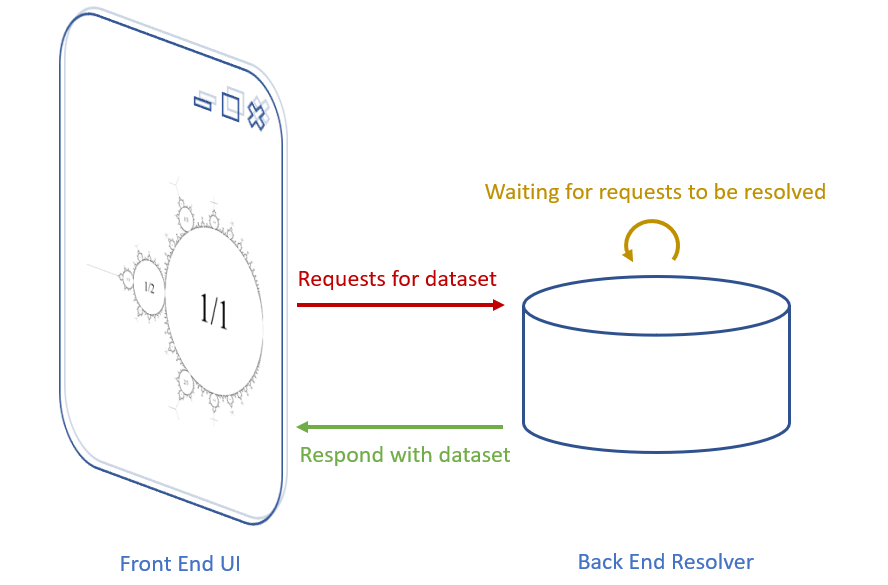
\includegraphics[width=.9\textwidth,keepaspectratio]{Figures/Chapter3/frontandback.png}
% 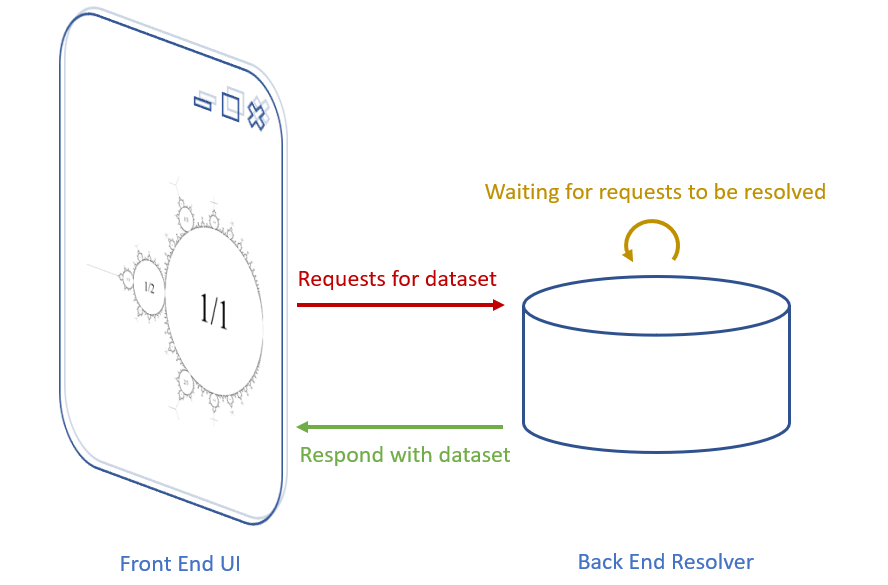
\includegraphics{Figures/Chapter3/frontandback.png}
\decoRule
\caption[Basic Structure]{ An illustration of the basic structure of the project, a front end that makes requests and a resolver that responds to the connected front end. }
\label{fig:frontandback}
\end{figure}

First of all, a front end \gls{ui} that organizes the content of the project, handling user interactions and so on, and making requests when some actual data of the extreme resolution dataset is needed.

Secondly, a back end resolver that resolves the requests coming from the connected front end, through necessary methods such as fetching an image from the database or calculate some values out of an equation. In the current state, however, this back end resolver should ``resolve'' the ``problem'' by calculation and not data fetching, calculating a portion of the dataset Mandelbrot set. It should return an image as an answer together with some necessary parameters so the front end can verify and use them as either a complete result image or as a intermediate buffer image, as shown in \gmref{fig:responsetypes}.

\begin{figure}[th]
\centering
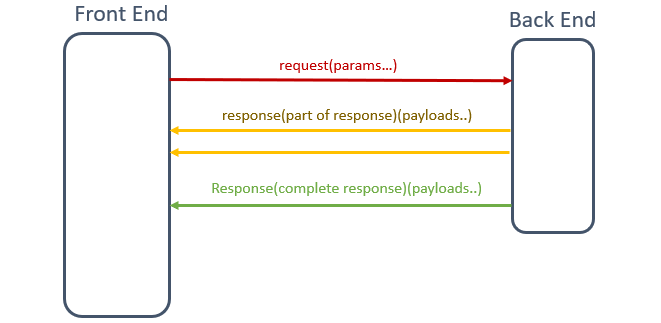
\includegraphics[width=.9\textwidth,keepaspectratio]{Figures/Chapter3/responsetypes.png}
% 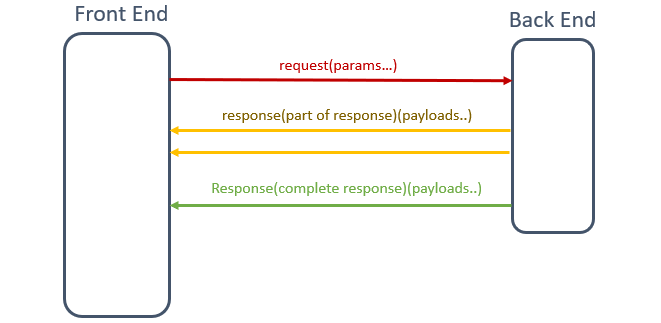
\includegraphics{Figures/Chapter3/responsetypes.png}
\decoRule
\caption[Different Reponse Types]{Responses of different types that the resolver can answer to the front end.}
\label{fig:responsetypes}
\end{figure}

%----------------------------------------------------------------------------------------
%	SECTION
%----------------------------------------------------------------------------------------

\section{Front End UI}

For starters, the front end should consist of three major parts: models of the \gls{fpc}, a manager to manage all these \glspl{fpc} and a effect manager to manage the effects to be displayed and some other \gls{ui} interactionss and controls from the user which in turn results to more effects.

First of all, let's look at the model of a pair of \gls{fpc}. This model should represent a tiny manager that manages one focus view together with a context view, as shown in \gmref{fig:fpcpair}. It's connected with these two targets and when it's being instructed to send messages to the outside world (not inside front end criteria), requests and receives responses and handle the render event, putting them on corresponding canvases.

\begin{figure}[H]
\centering
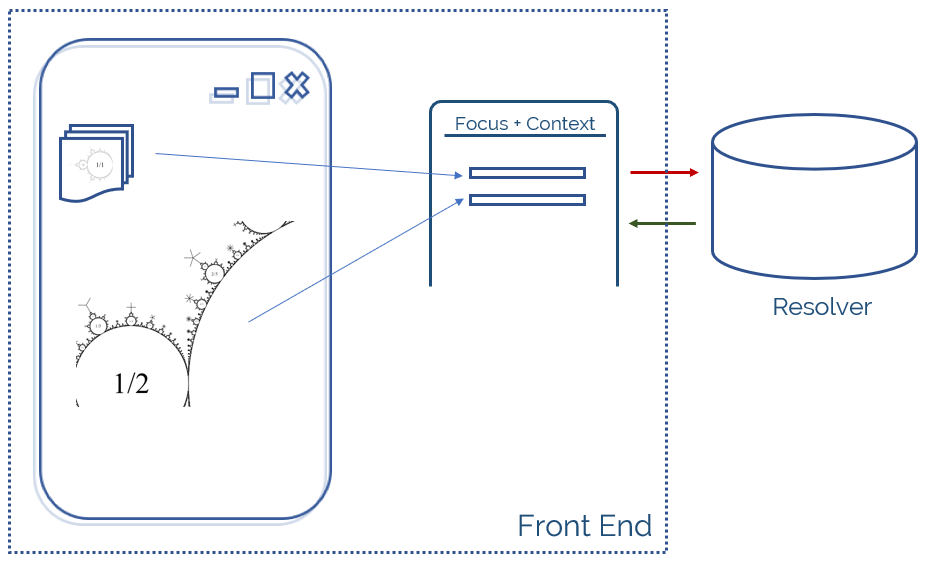
\includegraphics[width=\textwidth,keepaspectratio]{Figures/Chapter3/fpcpair.png}
% 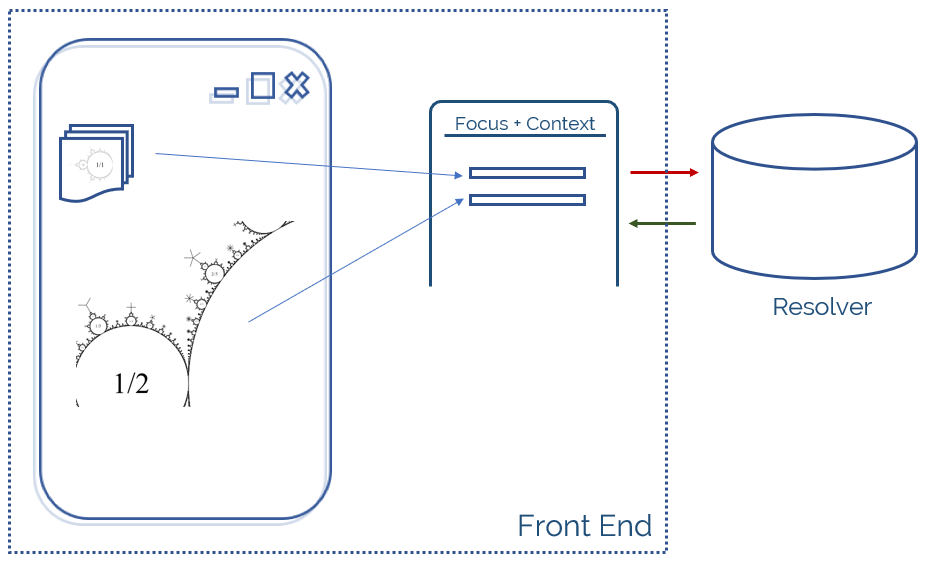
\includegraphics{Figures/Chapter3/fpcpair.png}
\decoRule
\caption[A Pair of Focus + Context]{Model of a pair of \gls{fpc}, a tiny manager that connects a focus view(the one in the center of the browser in this illustration) with a context view(the smaller view displaying dataset information), as well as sending pings to the outside.}
\label{fig:fpcpair}
\end{figure}

And then a single instance of that model is not enough, let's look at the manager that manages all generated \gls{fpc} models shown in \gmref{fig:fpcmanager}. We can see that this manager should manage the connections between each \gls{fpc} model with their corresponding canvases, as well as controlling them when to send or receive requests to the outside world, in turn controls the message exchange between the entire front end with the outside world resolver.

Note that from a insider point of view, this manager controls all the message exchange for all the \gls{fpc} models, however, to the outside world, this resolver is still handling all the different connections like treating multiple clients and don't have knowledge of the presence of this manager. Another thing that worth mentioning is that this manager should also handle the initializations of all the \gls{fpc} models. Non-effect based \gls{ui} events should also be handled here as some user interactions like zooming and panning require data exchange between the front end side and the outside world.

\begin{figure}[H]
\centering
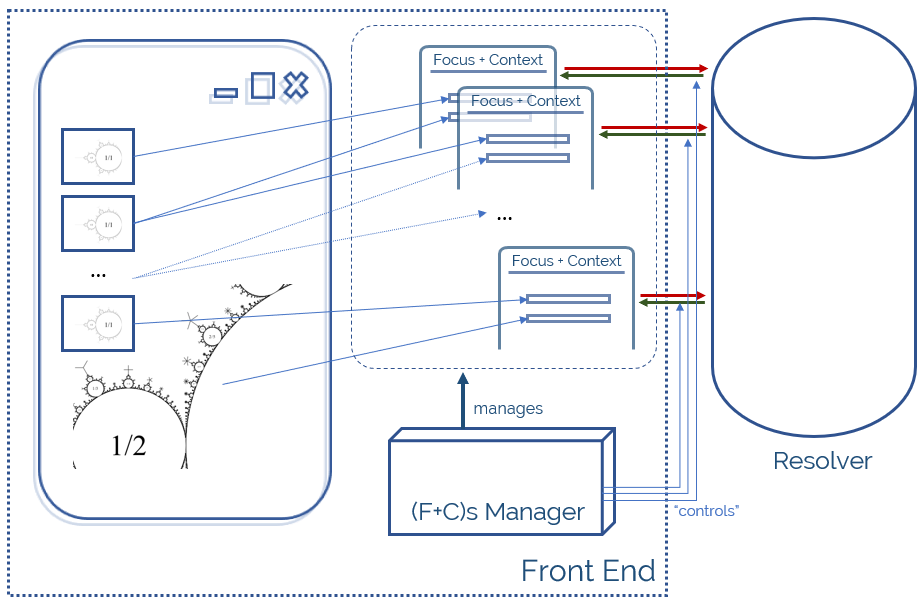
\includegraphics[width=\textwidth,keepaspectratio]{Figures/Chapter3/fpcmanager.png}
% 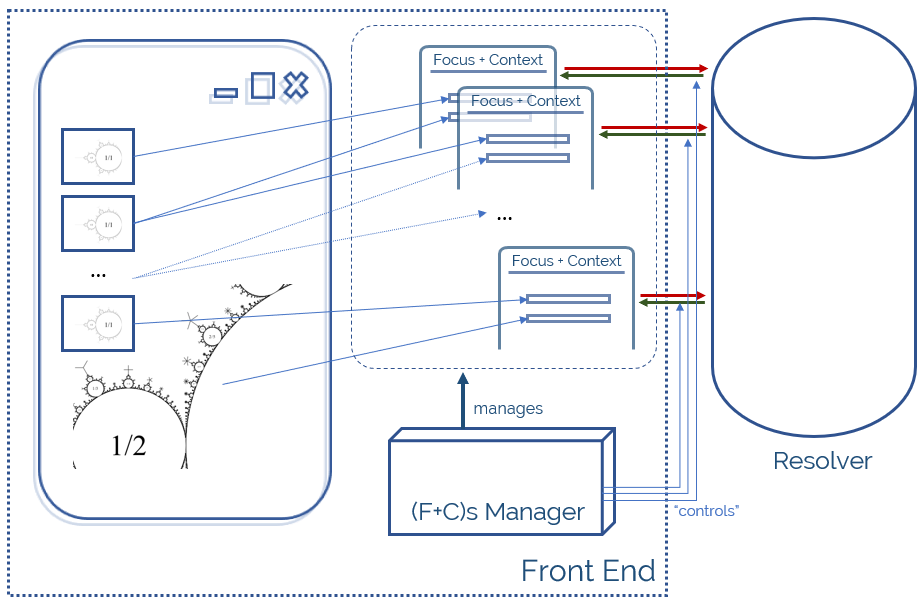
\includegraphics{Figures/Chapter3/fpcmanager.png}
\decoRule
\caption[Manager of All The F+Cs]{A manager that manages all the \gls{fpc} models that are connected properly with corresponding views and outside world, in turn controls the data exchange between the front end \gls{ui} with outside world.}
\label{fig:fpcmanager}
\end{figure}

Finally we need a manager that manages only the visual effects. All related affairs should be within the criteria of not requiring data exchange with the outside world, as shown in \gmref{fig:effectsmanager}. This manager will manage the arrangements of the \gls{fpc} models but only on the front end, for example the activation / deactivation of effects, the positions and visual effects occuring during these processes, and user interactions with the control panel that triggers rearrangements of the on-screen canvases, and the mechanics of previews.

It is worth mentioning that the preview mechanics, since it being purely on front end, is managed by this effect manager. This manager detects this user interaction when trying to activate one of the previews, and then goes into its storage and find corresponding recorded dataset data, finally instruct corresponding \gls{fpc} model to render them on the canvas that's for previewing purpose.

To summarize:

\begin{itemize}
    \item Manages \gls{fpc} models with respect to effects.
    \item Manages user interactions on \gls{fpc} models with respect to their context canvases and preview mechanics.
    \item Manages user interactions on control panels.
    \item Manages everything else that stays in front end criteria.
\end{itemize}

\begin{figure}[H]
\centering
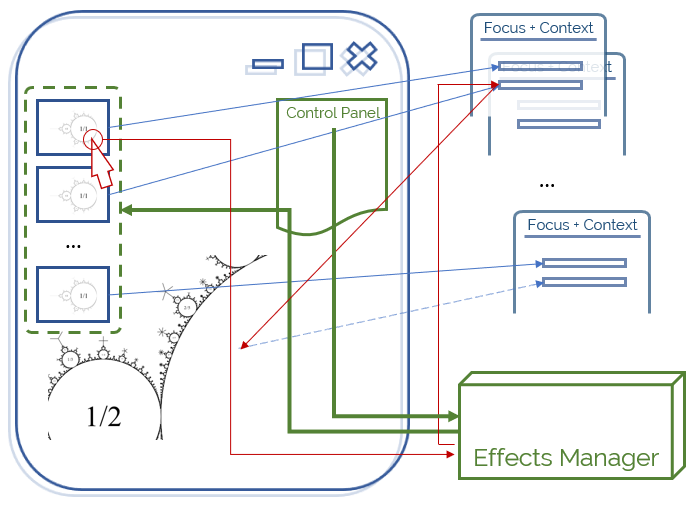
\includegraphics[width=0.85\textwidth,keepaspectratio]{Figures/Chapter3/effectsmanager.png}
% 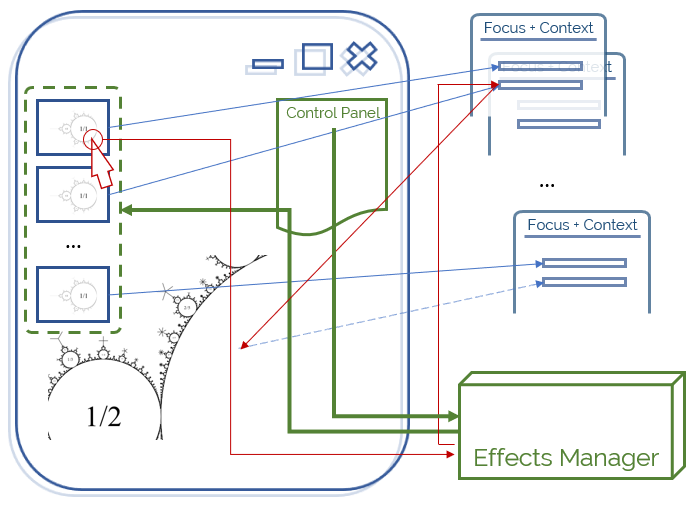
\includegraphics{Figures/Chapter3/effectsmanager.png}
\decoRule
\caption[Manager of Effects]{A manager that manages all effects related routines, including: (green) getting feedback of first hand user interactions from control panel and reflect back to the arrangements of the pile of \gls{fpc} models; (red) some other user interactions such as mouse hovering event triggering the preview mechanics of putting preview image data onto the browser.}
\label{fig:effectsmanager}
\end{figure}

%----------------------------------------------------------------------------------------
%	SECTION
%----------------------------------------------------------------------------------------

\section{Back End Resolver}

As for the back end resolver, it can be fairly simple or can be a complete cluster of servers or supercomputers to solve the response.

In the current state of the project, however, is a relatively simple script that compute for the required dataset with a given solution and location information, and send the results back to the front end, gracefully with the help of modern technology \gls{h5} introduced in \gmref{chap2:html5}.

The structure of it can be narrowed down to three essential part: 

\begin{itemize}
    \item Kickstarting of the idle state.
    \item Reception of requests, necessary parsing of the requests and sending them to calculation instances.
    \item Responses during the calculation / fetching process of the extreme resolution dataset, and / or at the end of the calculation / fetching as final results.
\end{itemize}